\documentclass[a4paper,14pt]{extarticle}
\usepackage[utf8]{inputenc}
\usepackage{multicol}
\usepackage[a4, total={6in, 8in}]{geometry}
\usepackage{listings}
\usepackage{graphicx}
\usepackage[export]{adjustbox}
\usepackage{tabularx}
\usepackage{hyperref}
\usepackage{movie15}
\usepackage{subfigure}
\usepackage{float}
\usepackage{listings}
\usepackage{xcolor}
\usepackage{tgpagella}

\definecolor{codegreen}{rgb}{0,0.6,0}
\definecolor{codegray}{rgb}{0.5,0.5,0.5}
\definecolor{codepurple}{rgb}{0.58,0,0.82}
\definecolor{backcolour}{rgb}{0.95,0.95,0.92}

\lstdefinestyle{mystyle}{
    backgroundcolor=\color{backcolour},   
    commentstyle=\color{codegreen},
    keywordstyle=\color{magenta},
    numberstyle=\tiny\color{codegray},
    stringstyle=\color{codepurple},
    basicstyle=\ttfamily\footnotesize,
    breakatwhitespace=false,         
    breaklines=true,                 
    captionpos=b,                    
    keepspaces=true,                 
    numbers=left,                    
    numbersep=5pt,                  
    showspaces=false,                
    showstringspaces=false,
    showtabs=false,                  
    tabsize=2
}

\lstset{style=mystyle}
\title{Side Notes on Practical Natural Language Processing: Bootstrap Test}
\author{Haritha G, Giridhar K}


\begin{document}
\maketitle

\section{Introduction}
Given a text classification task, we may often be interested in comparing the performance of various classifier systems. We want to know for instance, if adding an additional layer to the neural network improves the performance of the system. Just computing the metrics (accuracy, F-1 score, BLEU score etc.) in isolation are not sufficient to infer that the augmentation is increasing performance. In order to test whether an augmented system is better than the existing one, we use statistical tests to see whether the system is inherently better or the increase in performance is a chance occurrence. In the following sections we explain how we use one such non-parametric test called the \textit{bootstrap test} (also called as the permutation test). Note, in language processing, we don't generally use traditional statistical tests like the paired t-test to compare system outputs because most output metrics don't follow a normal distribution which violate their assumptions. 

\section{Concept explanation}
The word \textit{bootstrap} refers to the process of drawing repeated samples from a given set. Given a text classification problem and say we want to compare the performance of two classifiers $A$ and $B$ on a validation set $X_v$ containing $n$ elements, we start by defining our null and alternate hypotheses on the difference in performance between A and B, $\delta(X_v)$ as follows:
$$H_0: \delta(X_v) = 0 $$
$$H_1: \delta(X_v) > 0$$

If the performance of $A$ is the same as $B$ then \textit{we fail to reject the null hypothesis} that $\delta(X_v) = 0$. If one of the classifiers have a better performance then \textit{we reject the null hypothesis} that  $\delta(X_v) = 0$. As in, if we end up rejecting the null hypothesis, it means the probability of system $A$ having an accidental advantage over system $B$ is minimal. The performance of the two systems can now be compared by any metric that we may define. We illustrate the concept using \textit{accuracy} as our metric.

We test the hypotheses by repeatedly drawing random samples of size $n$ from the Validation set $X_v$, $b$ times and recording the performance metric in each case. We denote these sample point sets as $x^{*(i)}$ for $i=1...b$.
Now that we have a sampling distribution, we can do statistics of how often system $A$ has an accidental advantage in prediction over $B$. There are a number of ways to do that and we explain one such version.

We note that the recorded performance of $A$ and $B$ is centered at the expected value of $\delta(X_v)$. That is, about half the time $A$ will be better than $B$. In order to see if the performance of system $A$ exceeds $B$ by $\delta(X_v)$, we subtract this expected value and count the number of times $\delta(x^{*(i)}) > 2\delta(X_v)$.
This count is the number of times $A$ has an accidental advantage over $B$.  The ratio then acts as a one sided empirical p-value.
\begin{figure}[htp]
    \centering
    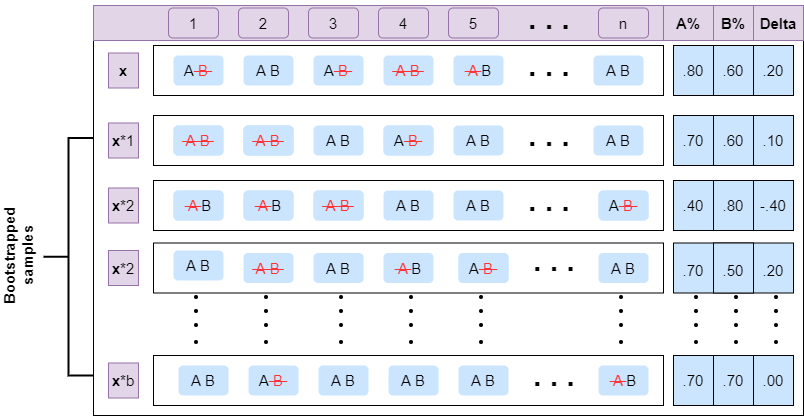
\includegraphics[width=14cm]{Bootstrap.png}
    \caption{Bootstrapping by drawing samples repeatedly and counting the number of times systems A and B have correctly or wrongly classified. The last 3 columns indicate the accuracy and their difference}
    \label{fig:galaxy}
\end{figure}
\section{Illustration of concept}
Here is a simple implementation on \textit{python} for two classifier systems $A$ and $B$. The size of the bootstrap sample $n$ is 10 and we draw $b= 100$ such samples $x^{*(1)}$ to $x^{*(100)}$. 


\begin{lstlisting}
def BOOTSTRAP(set_X, b): #returns p-value(x)
  d_X = np.sum(list(zip(*set_X))[0]) - np.sum(list(zip(*set_X))[1]) # how much better does algorithm A do than B on x
  d_X_1tob = [] 
  for i in range(0, b):
    A1_b, B1_b = (0, 0)
    # Draw a bootstrap sample x(i) of size n
    for j in range(len(set_X)):
      #Select a member of x at random and add it to x(i)
      set_Xb = random.choice(set_X) 
      A1_b += set_Xb[0]
      B1_b += set_Xb[1]
    d_X_1tob.append(A1_b - B1_b)  #delta: how much better does algorithm A do than B on x(i)
  
  #Count the samples on which algorithm A accidentally did better than B
  s = 0  
  for dx in d_X_1tob:
    if dx > (2 * d_X):
      s += 1    
  
  #onesided empirical p-value 
  p_val = s/b      
  return p_val

# Implementation 
real = [1,1,1,1,1,1,1,1,1,1]
A = [1,0,1,1,0,1,1,0,1,1] # system A
B = [1,1,0,0,0,1,1,0,1,0] # system B
b=100 # number of samples
def create_Input(real, A, B):
  A_pred = [0] * len(A)
  B_pred = [0] * len(B)
  for i, el in enumerate(real):
    if(real[i] == A[i]):
      A_pred[i] = 1
    if(real[i] == B[i]):
      B_pred[i] = 1
  return list(zip(A_pred, B_pred))

#Testing bootstrap
print(BOOTSTRAP(create_Input(real, A, B), b))
\end{lstlisting}

\section{References}
\begin{itemize}
    \item Daniel Jurafsky, James H. Martin, Speech and Language Processing: An Introduction to Natural Language Processing, Computational Linguistics, and Speech Recognition; Third Edition draft Oct 16, 2019.
    \item Fred Ramsey, Daniel Schafer, The Statistical Sleuth: A Course in Methods of Data Analysis, 3rd Edition


\end{itemize}

\end{document}
